%----------------------------------------------------------------------------------------
%	PACKAGES AND DOCUMENT CONFIGURATIONS
%----------------------------------------------------------------------------------------

\documentclass[10pt,a4paper]{article}

\usepackage[utf8]{inputenc}
\usepackage[spanish]{babel}
\usepackage{siunitx} % Provides the \SI{}{} and \si{} command for typesetting SI units
\usepackage{graphicx} % Required for the inclusion of images
\graphicspath{ {images/} }
\usepackage{natbib} % Required to change bibliography style to APA
\usepackage{amsmath}
\usepackage{amsfonts, amssymb} %Required for some math elements 
\usepackage{booktabs} %\toprule and tablas
\usepackage{hyperref}
\usepackage{rotating}
\usepackage{gensymb}
\usepackage{enumitem}
\usepackage{float}
\usepackage{colortbl}
\usepackage[margin=0.7in]{geometry}
\usepackage{cancel}
\usepackage{lipsum}% http://ctan.org/pkg/lipsum
\usepackage{fancyhdr}% http://ctan.org/pkg/fancyhdr
\usepackage{multirow}
\usepackage[table,xcdraw]{xcolor}
%\setlength\parindent{0pt} % Removes all indentation from paragraphs
\renewcommand{\labelenumi}{\alph{enumi}.} % Make numbering in the enumerate environment by letter rather than number (e.g. section 6)

\usepackage{times} % Uncomment to use the Times New Roman font

\usepackage{authblk} % author package
\renewcommand*{\Authand}{, } % para separar los autores por comas

\newcolumntype{P}[1]{>{\centering\arraybackslash}p{#1}}
\newcolumntype{M}[1]{>{\centering\arraybackslash}m{#1}}

\usepackage{makecell}%To keep spacing of text in tables
\setcellgapes{4pt}%parameter for the spacing


% to use tables visit http://www.tablesgenerator.com/latex_tables
\usepackage{multirow} % para usar multiples filas en una tabla

\setlength{\parindent}{0cm}
\def\thesubsection{\roman{subsection}}
\def\thesubsubsection{\alph{subsubsection}}

\newcommand\NP{97490}

%----------------------------------------------------------------------------------------
%	DOCUMENT INFORMATION
%----------------------------------------------------------------------------------------

\title{%
  Análisis Numérico - TP 2 \\
  \large Métodos numéricos aplicados a la Ingeniería de procesos}

\author{Rocío Gallo, padrón 97490 (rochimgg@gmail.com)\\ Facundo Monpelat, padrón 92716 (facundo.monpelat@gmail.com)}

\date{\today} %Date for the report


\begin{document}
%\begin{centering}
%\begin{align*}
% &Rocío Gallo, &&padrón 97490 &&(rochimgg@gmail.com)\\
 %&Facundo Monpelat, &&padrón 92716 &&(facundo.monpelat@gmail.com)
%\end{align*}

\maketitle % Insert the title, author and date

\section{Introducción}
Uno de los procesos más comunes de la industria metalúrgica es el tratamiento térmico de
aceros. Este tratamiento térmico le dará al acero diversas propiedades mecánicas en el cual el trabajo se enfocará a calcular solamente el tratamiento de Revenido. Este trabajo consiste en emplear métodos numéricos para encontrar resoluciones a una ecuación diferencial del calor que da la pauta, por ejemplo, de cuanto tiempo deberá estar el acero (en este caso un tubo) en el horno bajo ciertas temperaturas.

\definecolor{Gray}{gray}{0.85}

\section{Objetivos}
\begin{enumerate}
\item Experimentar el uso de métodos numéricos para la resolución de ecuaciones diferenciales
no lineales.
\item Aplicar métodos numéricos de diferentes temas de la materia y ensamblarlos para
resolver un problema de mayor complejidad.
\item Adquirir conocimientos básicos de la ingeniería de procesos industriales.
\end{enumerate}

\section{Desarrollo}
El intercambio de calor entre un sólido y su entorno está dado por la ley de conservación de
energía bajo la siguiente expresión:

\begin{equation}
\nonumber -mc\dfrac{dT}{dt}=h_{c}S(T-T_{\infty})+\gamma \Epsilon S(T^{4}-T_{\infty}^{4})
\end{equation}

donde el primer término representa el intercambio de calor debido al proceso de convección, mientras que el segundo término representa el intercambio de calor debido a la radiación.

\subsection{Métodos de resolución}
Para plantear los métodos, se acomodó la ecuación diferencial de la siguiente forma\\

\begin{equation}
\left\{ 
\begin{array}{ll}
T'=\dfrac{-h_{c}S(T-T_{\infty})}{mc}\\[10pt]
T_{0}= 293.5 K \\[10pt]
\end{array} \right.
\end{equation}

\subsubsection{Método de Euler}
Para este método la iteración viene dada por la expresión explícita:

\begin{equation}
\notag T_{i+1}=T_{i}+hT'(T_{i},t(i))
\end{equation}

El valor de $h$ es el tiempo de permanencia de un tubo en cada uno de los espacios que hay dentro del horno de revenido.

El $h$ puede ser calculado mediante la siguiente expresión:

\begin{equation}
\notag h = \dfrac{t_{Per}}{N_{Espacios}}\\[10pt]
\end{equation}

donde $t_{Per}$ es el tiempo de permanencia de cada tubo en el horno de revenido y $N_{Espacios}$ es la cantidad de espacios para tubos dentro del mismo horno.\\

La función escrita en python que implementa este método es:
\begin{verbatim}
#----------------------------------------------------------
# FUNCION euler(f,g,h,x0,xf,y0,data):
#
# PARAMETROS
# f:       Funcion de EDO
# g:       Funcion solucion analitica (Calculo de error)
# h:       Incremento o cadencia
# x0 y y0: Valores iniciales
# xf :     Valor final
# data :   Array de diccionarios que contiene los datos X e Y de cada iteracion
# USO      Calcula los valores con el metodo de Euler
#-----------------------------------------------------------
def euler(f,g,h,x0,xf,y0,data):
    t = x0
    y = y0
    i=0
    while t <= xf:
        delta = abs( y-g(t) )/g(t)
        aux_dict={
        'i':i,
        'X':t,
        'Y':y,
        'E':delta,
        }
        data.append(aux_dict)
        i=i+1
        y += h * f(t,y)
        t += h
    return data[-1]['X'],data[-1]['Y']
\end{verbatim}




\subsubsection{Método de Runge-Kutta Orden 4}
Para el calculo de este método se utilizaron las expresiones:
\begin{equation}
\left\{ 
\begin{array}{ll}
\notag k_{1} = f(t_{0}, T_{0})\\ [10pt]
\notag k_{2} = f(t_{0} + \dfrac{h}{2}, T_{0} + h\;(\dfrac{k_{1}}{2}))\\ [10pt]
\notag k_{3} = f(t_{0} + (\dfrac{h}{2}), T_{0} + h\;(\dfrac{k_{2}}{2}))\\ [10pt]
\notag k_{4} = f(t_{0} + h, T_{0} + h\;k_{3})\\ [10pt]
\end{array} \right.
\end{equation}
donde $t_{0}$ es las semilla de la variable tiempo (en segundos) y $T_{0}$ es la semilla de la variable temperatura (en Kelvin).\\
En los programas creados para este trabajo se las renombro de la forma:
$t_{0}\;=\;x_{0}$ y $T_{0}\;=\;y_{0}$.\\
La iteración de Runge - Kutta con estos coeficientes viene dada por la expresión:

\begin{equation}
\notag T_{n+1} = T_{n} + \dfrac{h}{6}\;(k_{1} + 2\;k_{2} + 2\;k_{3} + k_{4})\\
\end{equation}

La función escrita en python que implementa este método es:

\begin{verbatim}
#----------------------------------------------------------
# FUNCION rungeKutta(f,g,h,x0,xf,y0,data,i)
#
# PARAMETROS
# f:       Funcion de EDO
# g:       Funcion solucion analitica (Calculo de error)
# h:       Incremento o cadencia
# x0 y y0: Valores iniciales
# xf :     Valor final
# data :   Array de diccionarios que contiene los datos X e Y de cada iteracion
# i :      Contador de iteraciones 
# USO      Calcula los valores con el metodo de Runge-Kutta
#-----------------------------------------------------------

def rungeKutta(f,g,h,x0,xf,y0,data,i):
    debug = 0
    # K1 = F(Xn,Yn)
    # K2 = F( Xn + h/2 , Yn + h*K1 /2 )
    # K3 = F( Xn + h/2 , Yn + h*K2 /2 )
    # K4 = F( Xn + h/2 , Yn + h*K3 )
    k1 = f(x0, y0)
    k2 = f(x0 + (h/2), y0 + h*(k1/2))
    k3 = f(x0 + (h/2), y0 + h*(k2/2))
    k4 = f(x0 + h, y0 + h*k3)
    # Yn+1 = Yn + h/6( K1 + 2K2 + 2K3 + K4 )
    
    y = y0 + (h/6)*(k1 + 2*k2 + 2*k3 + k4)
    delta = abs( y0-g(x0) )/g(x0)

    aux_dict={
        'i':i,
        'X':x0,
        'Y':y0,
        'E':delta
    }

    if debug: pprint(aux_dict)

    data.append(aux_dict)

    if( round(x0) == xf ):
        if debug: print('X final: ' + str(data[-1]['X']) + '/ Y final: '+str(data[-1]['Y']) ) 
        return data[-1]['X'],data[-1]['Y']

    else:
        return rungeKutta( f, g, h, x0+h, xf, y, data, i+1)
\end{verbatim}


\subsection{Ejercicio 1}
Resolver el modelo planteado considerando solamente el intercambio de calor por convección. Aplicar los métodos de Euler y Runge Kutta de orden 4 para una condición inicial
$T_{0}=\SI{20}{\degree C}$ y paso de tiempo $h = cadencia$. \\
Para los cálculos se utilizo el número de padrón de Roció Gallo (\NP).

\begin{center}
\begin{tabular}{ |c|c|c| } 
\hline
\multirow{2}{*}{\centering Propiedades del
material}
& $\rho$ & $\SI{7850}{\kg\per\meter^2}$ \\ \cline{2-3}
& C & \SI{480}{\joule\per{\kg\kelvin}} \\ \cline{2-3}
\hline
\multirow{3}{*}{\centering Geometría del
material}
& $OD$ & $\SI{0.24448}{\meter}$ \\ \cline{2-3}
& $WT$ & $\SI{0.01384}{\meter}$ \\ \cline{2-3}
& $Lt$ & $\SI{12}{\meter}$ \\ \cline{2-3}
\hline
\multirow{2}{*}{\centering Geometría del horno}
& $L$ & $\SI{50}{\meter}$ \\ \cline{2-3}
& $nbol$ & 50 \\ \cline{2-3}
\hline
\multirow{3}{*}{\centering Parámetros de
proceso}
& $cad$ & $ROUND(\SI{-10}{\sec}  / 10000 * (\NP  - 90000) + \SI{35}{\sec})=\;28\;\si{\sec}$ \\ \cline{2-3}
& $T_{1}$ & $ROUND(\SI{200}{\degree C} / 10000 * (\NP - 90000) + \SI{500}{\degree C} )=\;650\si{\degree C}$\;=\;\SI{923.15}{\kelvin} \\ \cline{2-3}
& $T_{2}$ & $ROUND( \SI{200}{\degree C} / 10000 * (\NP - 90000) + \SI{500}{\degree C} )=\;650\si{\degree C}$\;=\;\SI{923.15}{\kelvin} \\ \cline{2-3}
\hline
\multirow{3}{*}{\centering Parámetros de la
transferencia de calor}
& $hc$ & $\SI{20}{\watt\per{\meter^2\kelvin}}$ \\ \cline{2-3}
& $\sigma$ & $5.6703\;10^{-8}\si{\watt\per{\meter^2\kelvin^4}}$\\ \cline{2-3}
& $\epsilon$ & 0.85 \\ \cline{2-3}
\hline
\end{tabular}
\end{center}

\\
Notar que para este caso particular donde $T_{\infty}=T_{1}=T_{2}$, la solución analítica (exacta) tiene la siguiente expresión:

\begin{equation}
\begin{split}
\nonumber T(t) = T_{\infty} + (T_{0}-T_{\infty})e^{\dfrac{h_{c}S}{mC}t}
\end{split}
\end{equation}

\begin{enumerate}
\item Graficar la temperatura en función del tiempo superponiendo los resultados de cada método junto con la solución exacta.
\item Graficar el error relativo cometido con cada método en función del tiempo. Utilizar una escala en el eje vertical que permita visualizar con claridad ambas curvas.
\item Obtener conclusiones sobre la precisión de ambos métodos aplicados.
\end{enumerate}

IMPORTANTE: Los cálculos de temperatura y tiempo asociados a la ecuación diferencial deberán realizarse en grados Kelvin [$\si{\kelvin}$] y segundos [$\si{\sec}$], respectivamente. Por otro lado, los resultados (ya sean numéricos o plasmados en gráficos) deberán expresarse en grados Celsius [$\si{\degree C}$] y minutos [$\si{\min}$].\\
\\
Sabiendo que la superficie es:
\begin{equation}
\begin{split}
\nonumber S = \pi\;OD\;L_{t}\;=\;\SI{9.2167}{\meter^2}
\end{split}
\end{equation}
y la masa:
\begin{equation}
\begin{split}
\nonumber m = \rho\;\pi\;OD\;WT\;(1-\dfrac{WT}{OD})\;L_{t}=\;\SI{944.6512}{\kg}
\end{split}
\end{equation}

\newcommand\masa{944.6512}
\newcommand\superficie{9.2167}

\newcommand\tone{650}
\newcommand\ttwo{650}

La ecuación a resolver con $T_{0}=\SI{20}{\degree C}=\SI{293.15}{\kelvin}$ es:
\begin{equation}
\begin{split}
T'=-4.0631\;10^{-4}(T-T_{\infty})\\
T'=-4.0631\;10^{-04}\;(T-923.15)
\end{split}
\end{equation}

Se resuelven ambos métodos creando un script en python. Se ejecuta el código y este abre 2 ventanas en un navegador predeterminado con los gráficos.\\
Ejeccucion:
\begin{verbatim}
Skywalker:EJ1 fmonpelat$ python3.7 TP2-ej1.py
Datos calculados: 
m [kg] = 945.9618816430382
S [m2] = 9.228742579185376
Cadencia [seg] : 28.0
v_0 [m/s] = 0.03571428571428571
\end{verbatim}

La gráfica comparativa de los métodos con respecto a la solución analítica es la siguiente: 
\begin{figure}[H]
\centering
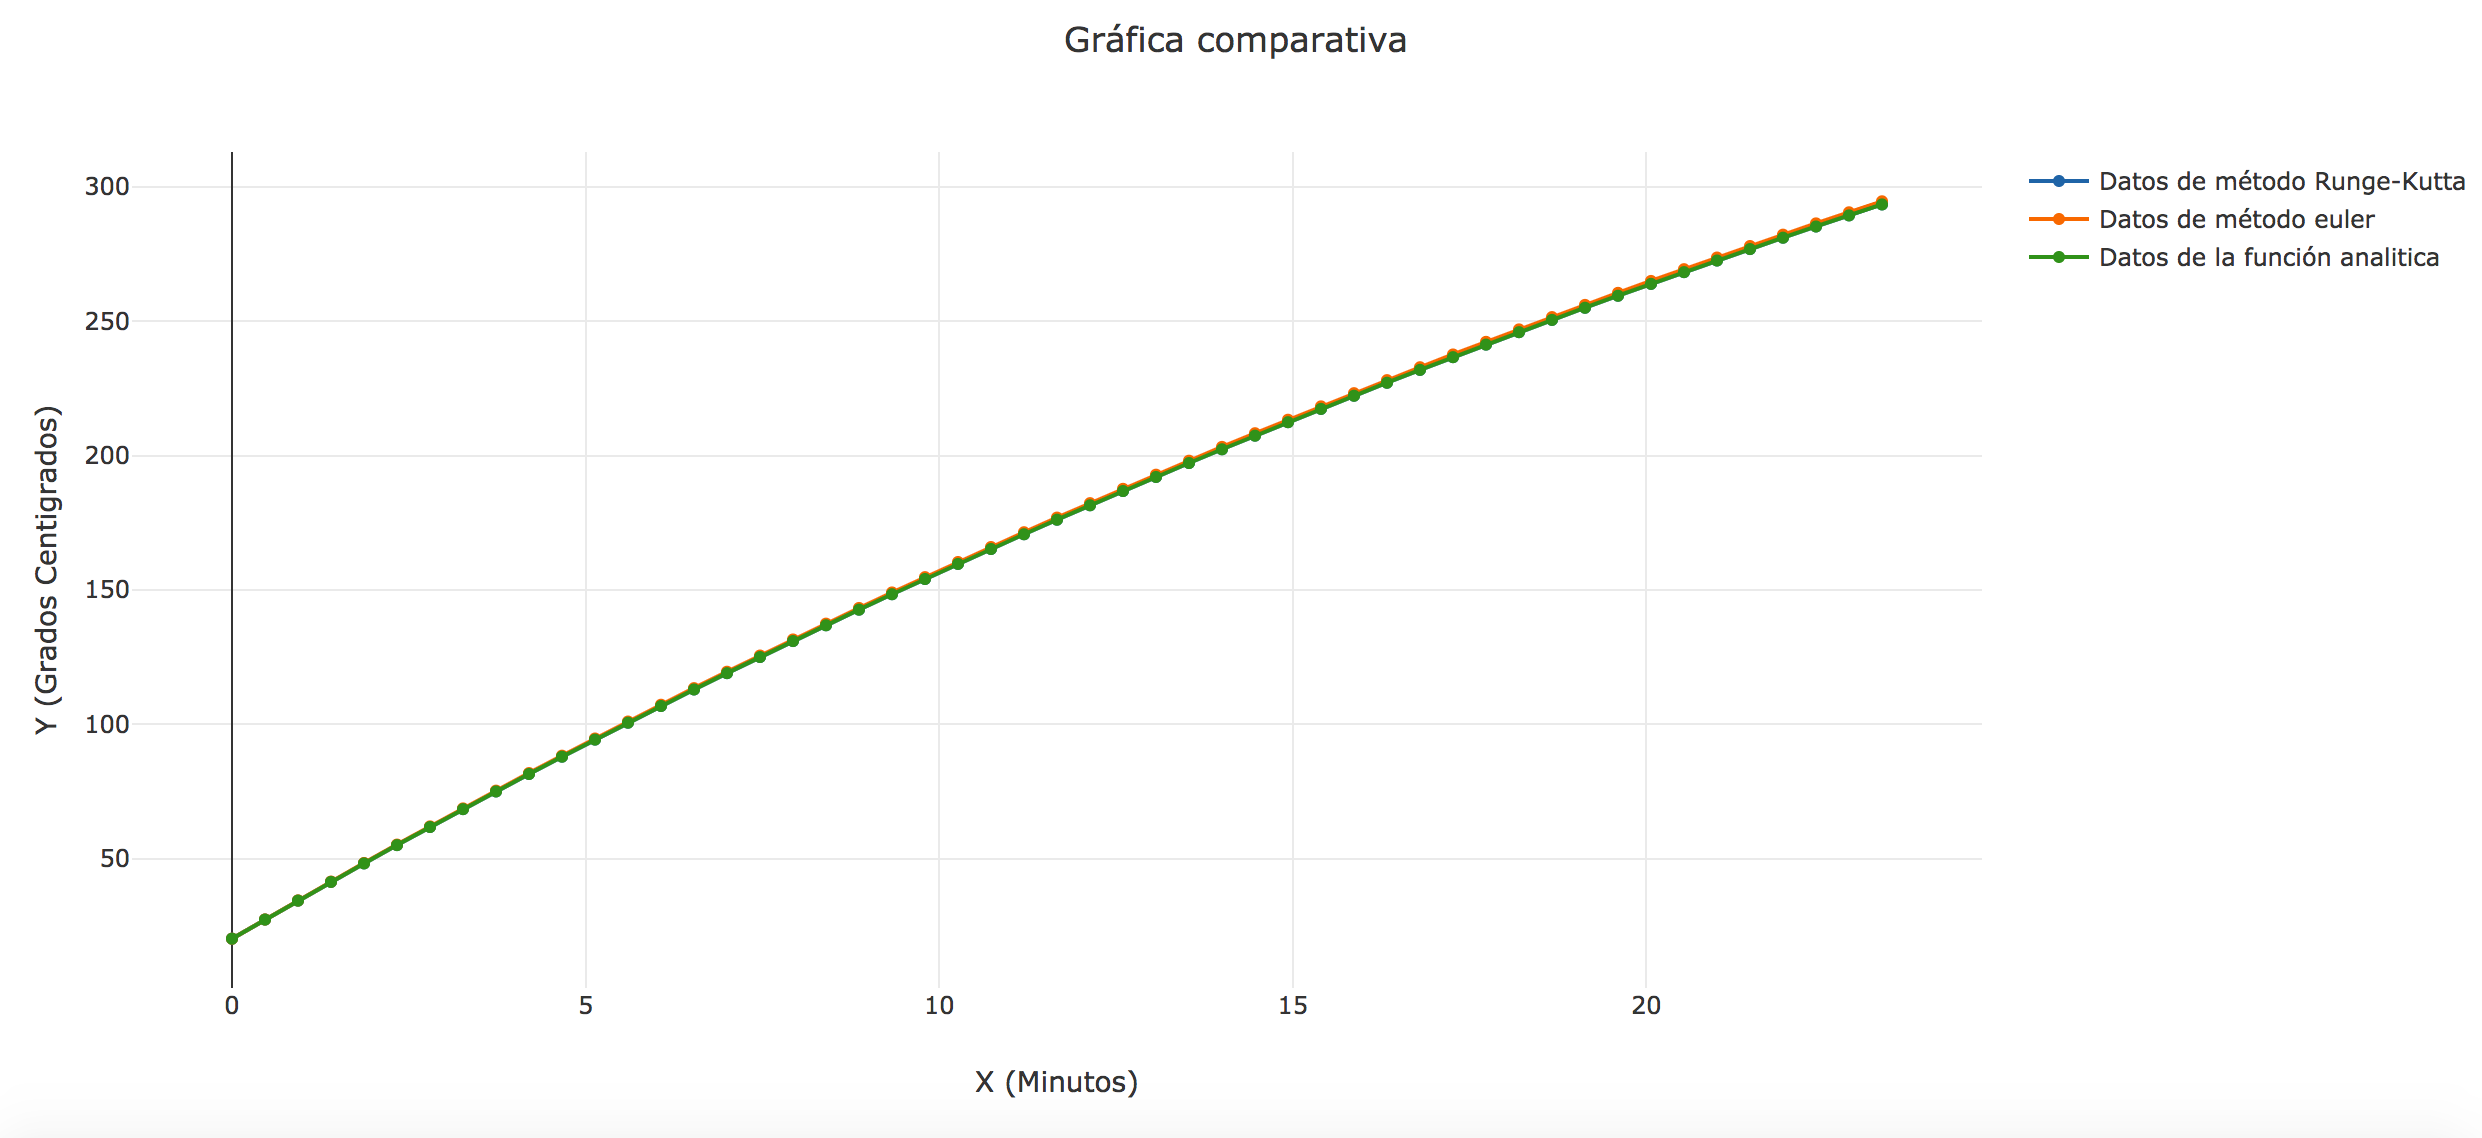
\includegraphics[width=15cm]{Grafica-ej1.png}
\caption{Comparativa entre métodos.}
\end{figure}

y la imagen que muestra los errores de cada método con escala vertical logarítmica es:
\begin{figure}[H]
\centering
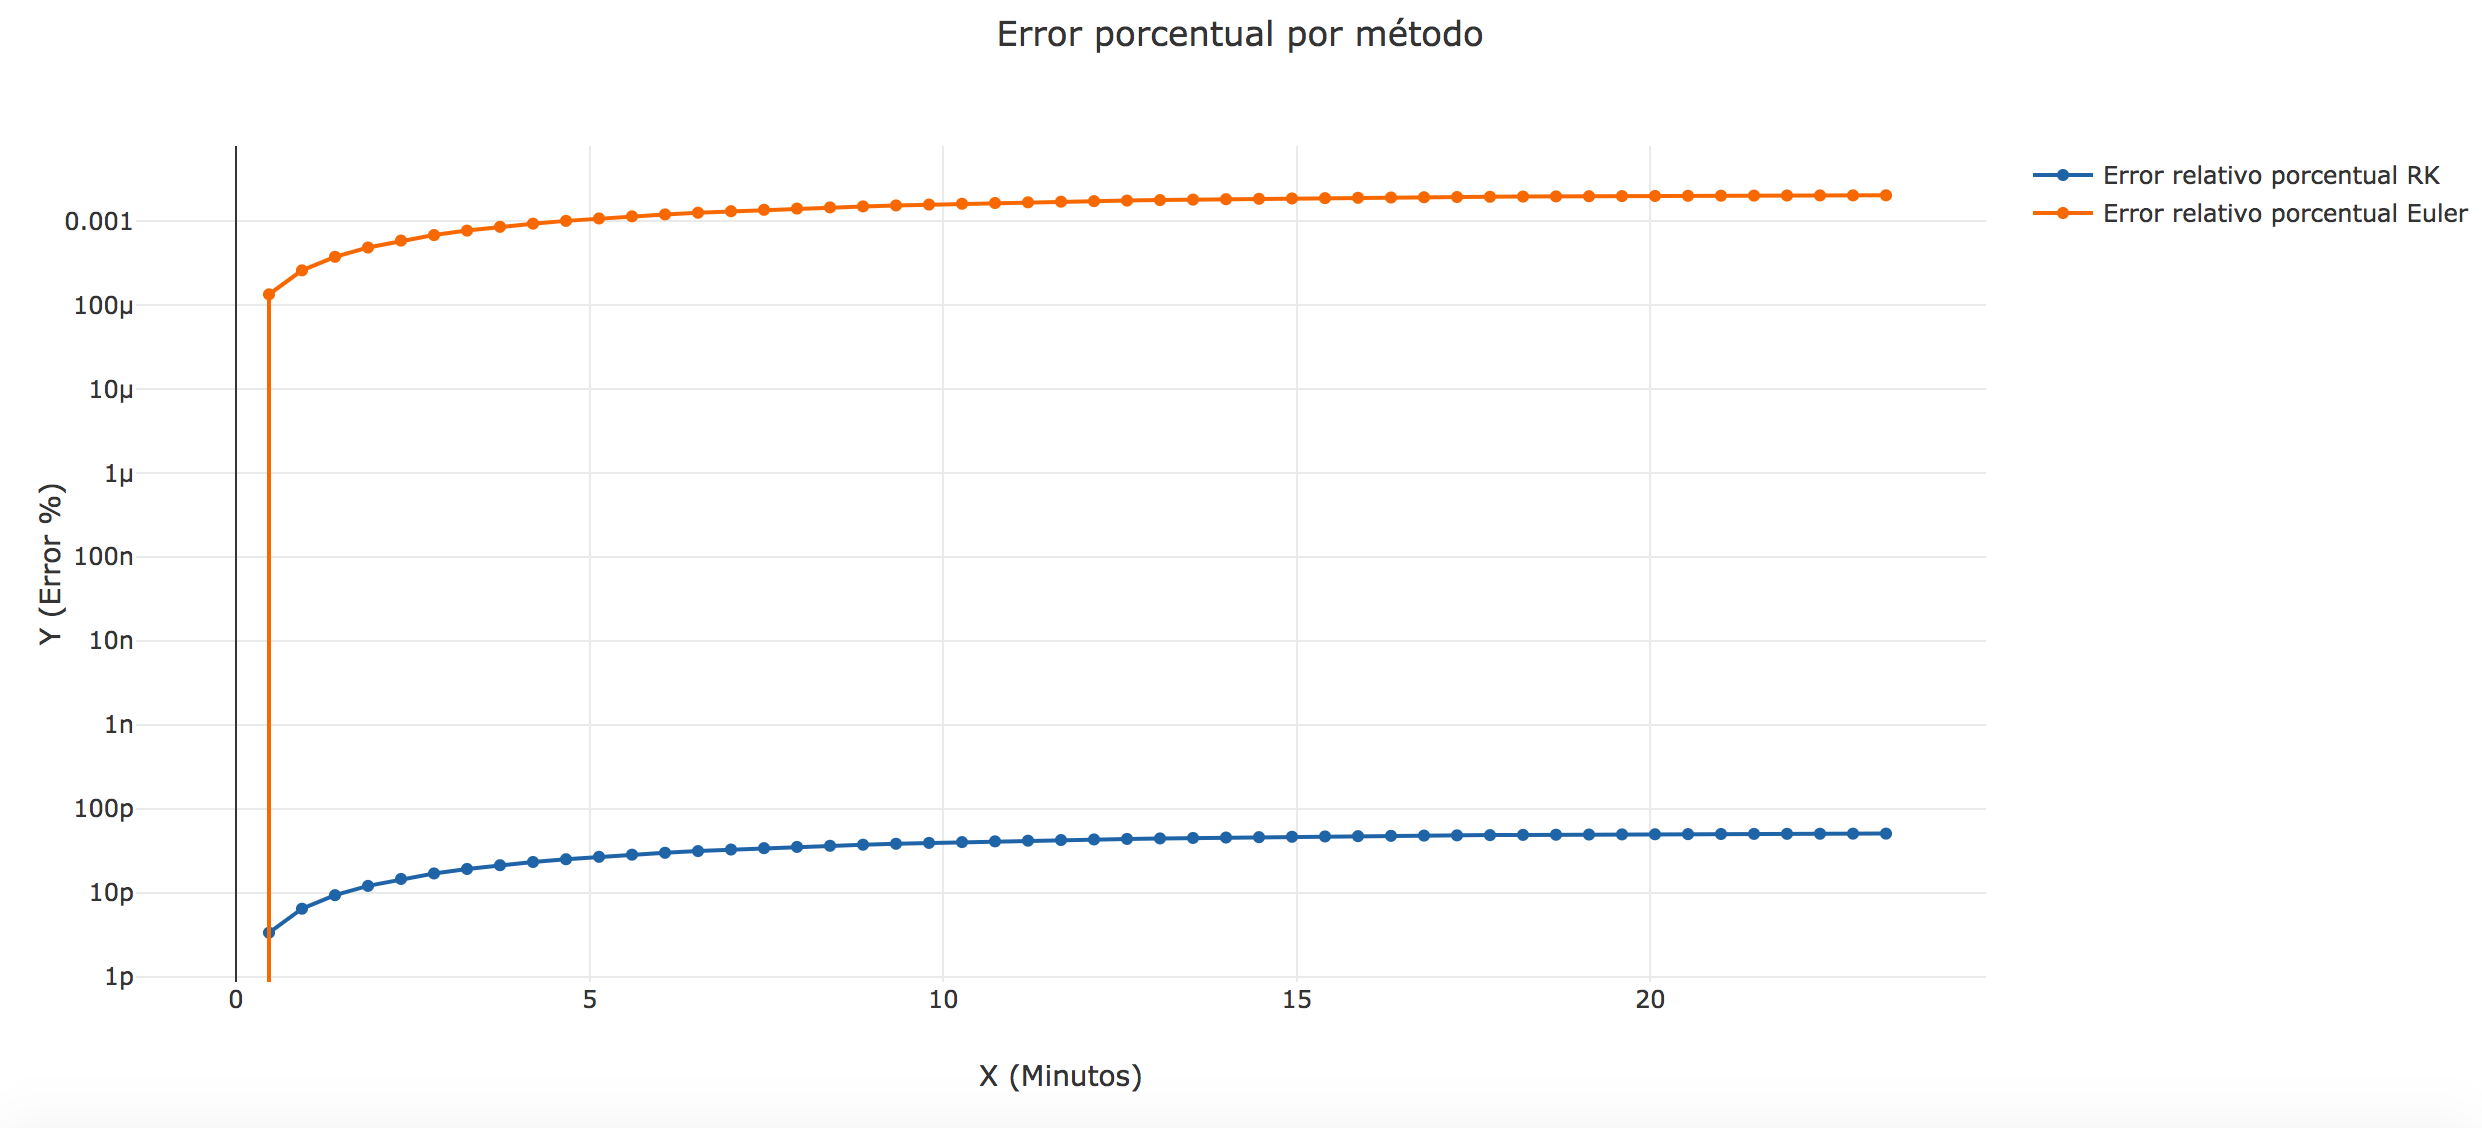
\includegraphics[width=15cm]{Errores-ej1.png}
\caption{Comparativa entre métodos.}
\end{figure}

Se nota que los errores con respecto a la solución analítica son mas apreciables con Euler que con el método de Runge-Kutta. Uno esta en el rango de los micro y el otro en el rango de los pico y por este motivo se puede afirmar que el método de Runge-Kutta es mas preciso.



\subsection{Ejercicio 2}
\subsubsection{Elección}
Para hacer el análisis de la ecuación de conservación de energía con ambos términos se optará por utilizar el método numérico de Runge-Kutta de orden 4.  Cómo se ha visto en el primer punto, la distancia entre la gráfica analítica y la aproximada mediante Runge-Kutta es significativamente menor que la obtenida mediante el método de Euler y por lo tanto mas precisa.\\

Para resolver este punto se creó otro script en python donde su ejecución fue la siguiente:
\begin{verbatim}
Skywalker:EJ2 fmonpelat$ python3.7 TP2-ej2.py 
Datos calculados: 
m [kg] = 945.9618816430382
S [m2] = 9.228742579185376
Cadencia [seg] : 28.0
v_0 [m/s] = 0.03571428571428571
Tsk(K):  874.613710100969 K
Tsk(C):  601.613710100969 C
Sk(seg):  224.0 seg
Sk(min):  3.7333333333333334 min
\end{verbatim}
y la gráfica fue la siguiente:
\begin{figure}[H]
\centering
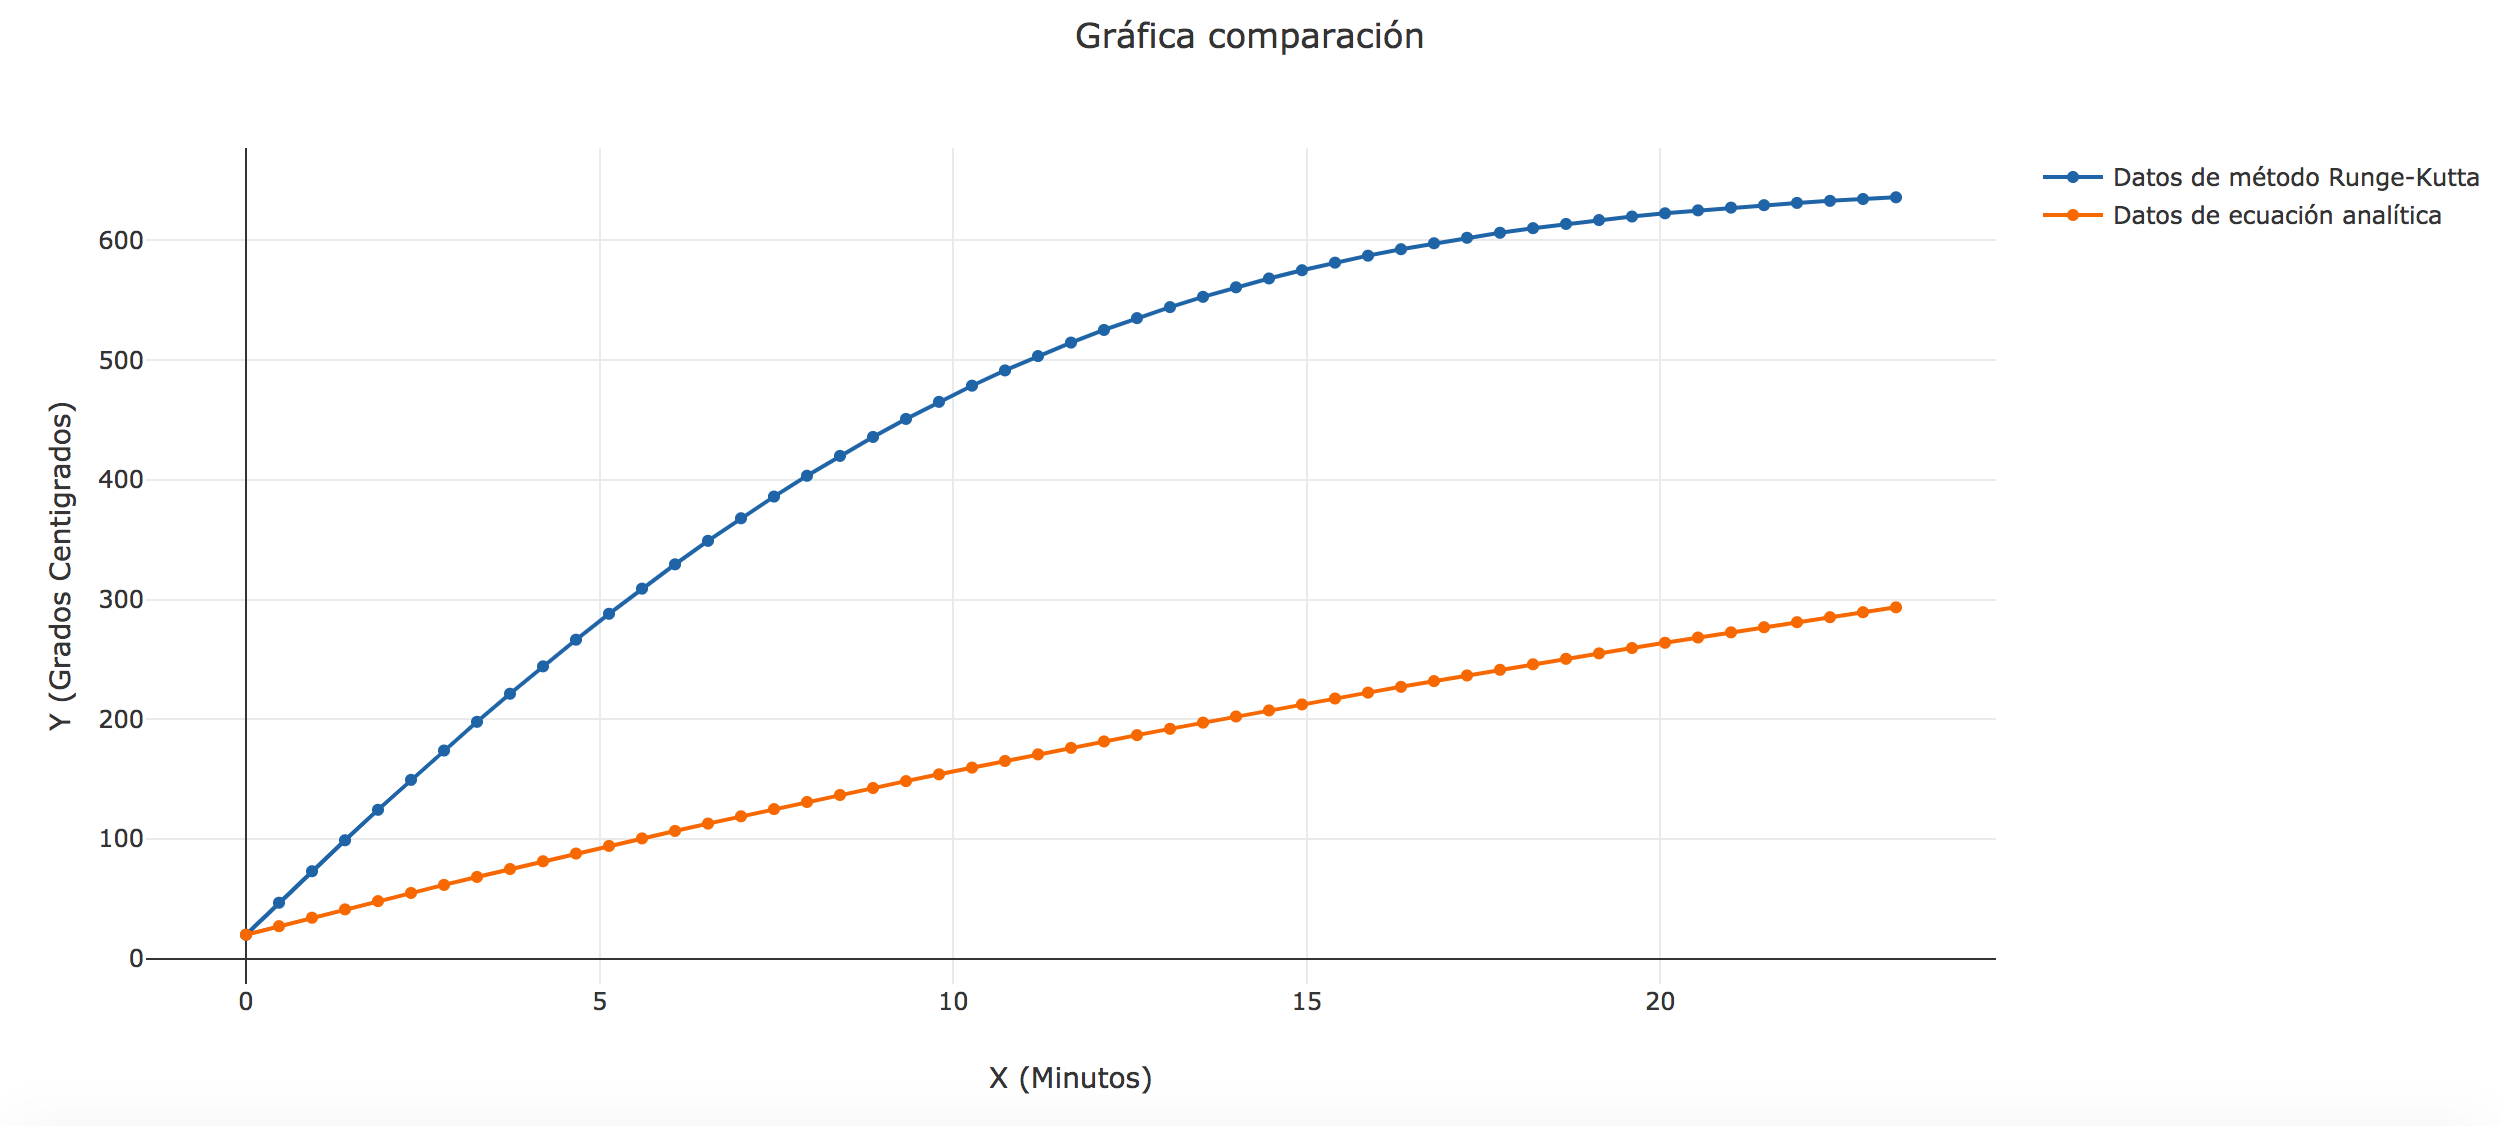
\includegraphics[width=18cm]{Grafica-ej2.png}
\caption{Solución RK con intercambio radiativo y solución analítica sin intercambio radiativo.}
\end{figure}
Como se puede ver en la gráfico el intercambio por radiación no es despreciable.
El código retornó la temperatura media en el tiempo de soaking y su tiempo correspondiente:
Tsk(K):  874.613 Kelvin
Tsk(C):  601.613 Centigrados

Sk(seg):  224.0 segundos
Sk(min):  3.733 minutos

\subsection{Ejercicio 3}
Este ejercicio pide encontrar manualmente una combinación de $T_{1}$ y $T_{2}$ para que el $S_{k}$ sea de 10 minutos
manteniendo la $T_{sk}$ obtenida en el ítem 2. La tolerancia para $S_{k}$ es de $\pm0.5min$.
\\
\\
Para resolverlo fue fijada la temperatura de soaking del ejercicio anterior $Tsk(\si{\kelvin}):\SI{874.613}{\kelvin}$.
Cambiando $T_{1}$ y $T_{2}$ manualmente e imprimiendo el tiempo en minutos para una temperatura próxima a $T_{sk}$ obtenemos con los valores:
$T_{1}$ = 1002 Kelvin y $T_{2}$= 922.5 Kelvin.
\begin{verbatim}
Skywalker:EJ3 fmonpelat$ python3.7 TP2-ej3.py 
Datos calculados: 
m [kg] = 945.9618816430382
S [m2] = 9.228742579185376
Cadencia [seg] : 28.0
v_0 [m/s] = 0.03571428571428571
Sk Objetivo [segundos] : 600
Tsk Objetivo [C] = 602
tiempo Sk: 10.267 [min] tiempo obj: 10.000 [min] temp mean: 606.066 [C] temp obj: 602.00 [C]
\end{verbatim}
como la tolerancia pedida es 0.5 minutos la medición que llegamos con esos valores cumple ($Sk=10.267-10=0.267\;minutos$).\\
La nueva gráfica que cumple lo pedido será:
\begin{figure}[H]
\centering
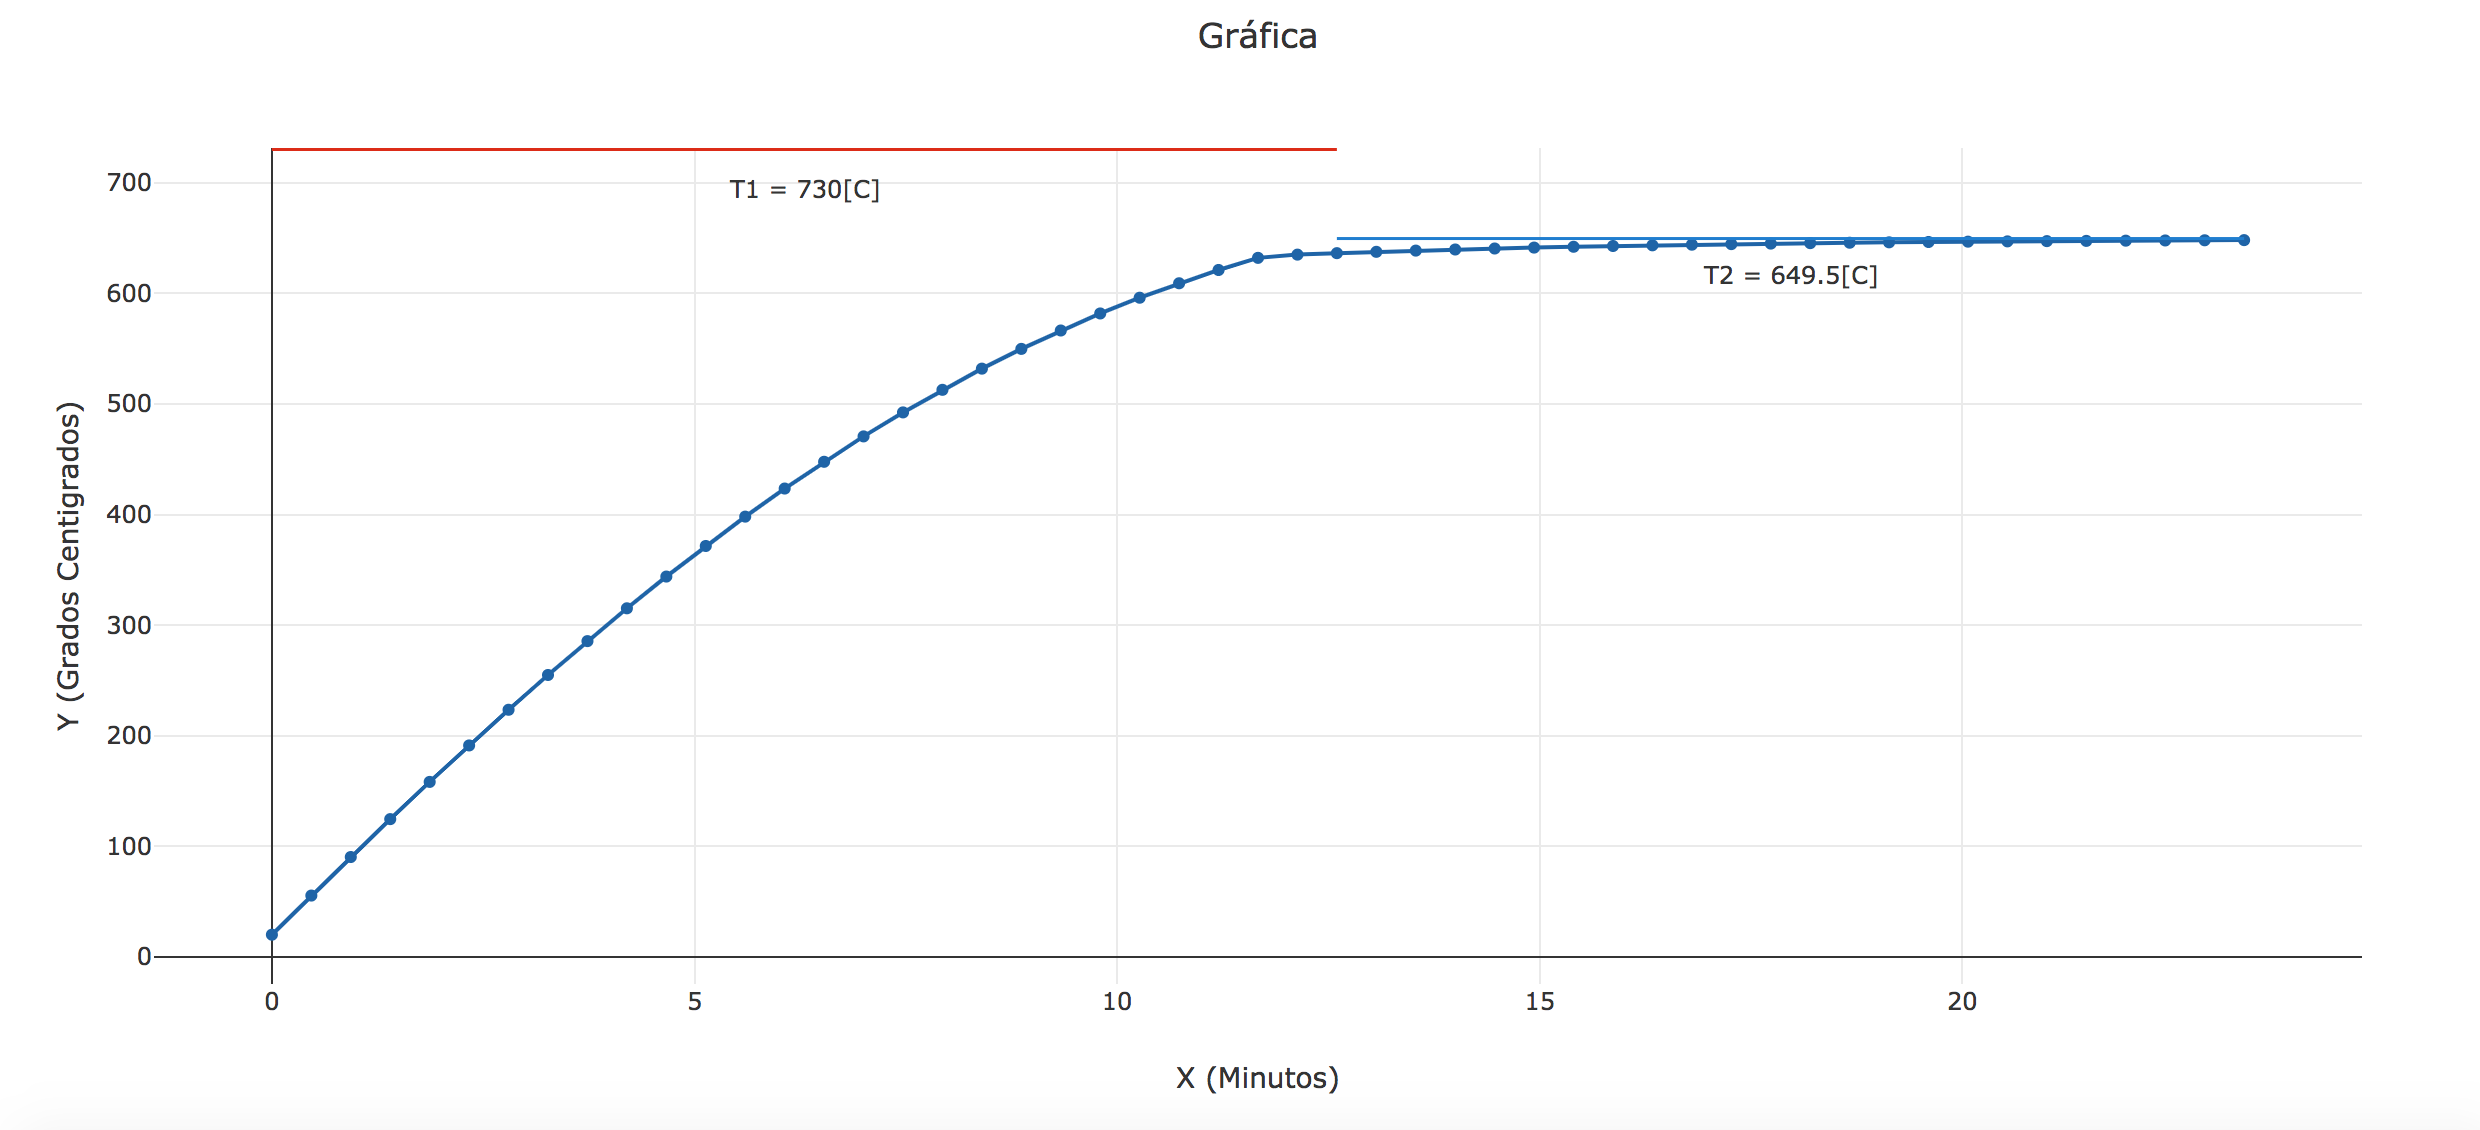
\includegraphics[width=18cm]{Grafica-soaking_ej3.png}
\caption{Solución númerica con los valores $T_{1}$ = 1002 Kelvin y $T_{2}$= 922.5 Kelvin}
\end{figure}


\subsection{Ejercicio 4}
Realizar una mejora del ciclo térmico obtenido en el ítem 3 en términos de productividad. Es decir, aumentar la productividad un 5\% sin alterar los parámetros metalúrgicos de interés (iguales valores de $S_{k}$ y $T_{sk}$).

\subsubsection{Algoritmo}

Para lograr un rendimiento un 5\% mayor será necesario llegar a los mismos $T_{Sk}$ y $S_{k}$ pero en un tiempo menor.\\

Para conseguir esto, se optó por multiplicar la cadencia de la consigna por $0,95$ y así obtener unas temperaturas $T_{1}$ y $T_{2}$ que corresponden a un rendimiento un 5\% mayor.Los valores obtenidos para $T_{1}$ y $T_{2}$ fueron\\

\[
\begin{array}{cc}
      T_{1}=846,93 C\degree \\
      T_{2}=722,733 C\degree\\
\end{array}
\]

Este punto fue realizado luego de plantear el inciso 5, porque era más directo el cálculo habiendo resuelto el problema del hallazgo automatizado de $T_{1}$ y $T_{2}$.


\subsection{Ejercicio 5}

\subsubsection{Algoritmo}

Para la resolución de este ejercicio, el enunciado propone utilizar un esquema de punto fijo con la siguiente matríz jacobiana

\[
   J=
  \left[ {\begin{array}{cc}
   0,25 & 0,75 \\
   0,75 & 0,25 \\
  \end{array} } \right]
\]

cuya inversa está dada por

\[
   J^{-1}=
  \left[ {\begin{array}{cc}
   -0,5 & 1,5 \\
    1,5 & -0,5 \\
  \end{array} } \right]\\
\]

Dado que $T_{Sk-obj}$ y $Sk_{obj}$ son las raices del modelo planteado anteriormente se plantea la siguiente iteración de punto fijo.\\

\[
  \left[ {\begin{array}{cc}
   T_{1}^{k+1}  \\
   T_{2}^{k+1}
  \end{array} } \right] =
   \left[ {\begin{array}{cc}
   T_{1}^{k}  \\
   T_{2}^{k}
  \end{array} } \right] -
  \left[ {\begin{array}{cc}
   -0,5 & 1,5 \\
    1,5 & -0,5 
  \end{array} } \right]
  \left[ {\begin{array}{cc}
   F_{1}(T_{1}^{k},T_{2}^{k})  \\
   F_{2}(T_{1}^{k},T_{2}^{k})
  \end{array} } \right]
\]

Donde $F_{1}$ y $F_{2}$ vienen dados por la siguiente expresión

\begin{align*}
    &F_{1}(T_{1},T_{2})= f_{1}(T_{1},T_{2}) - T_{Sk-obj}=0\\
    &F_{2}(T_{1},T_{2})= f_{2}(T_{1},T_{2}) - Sk_{obj}=0
\end{align*}

Luego de realizados los cálculos, fueron obtenidas las siguientes temperaturas $T_{1}$ y $T_{2}$ para cada caso solicitado.

\begin{table}[H]
     \makegapedcells
     \centering
\resizebox{0.5\textwidth}{!}{
         \begin{tabular}{|c|c|c|c|c|c|}
\hline Caso & Sk & Tsk & T1 & T2 & Iteración \\
\hline A & 10 & 602 & 860.382 & 708.72 & 62 \\
\hline B & 10 & 624.9 & 772.171 & 733.519 & 52 \\
\hline C & 10 & 674.9 & 666.048 & 776.556 & 36 \\
         \hline
     \end{tabular}}
\end{table}


\begin{figure}[H]
\centering
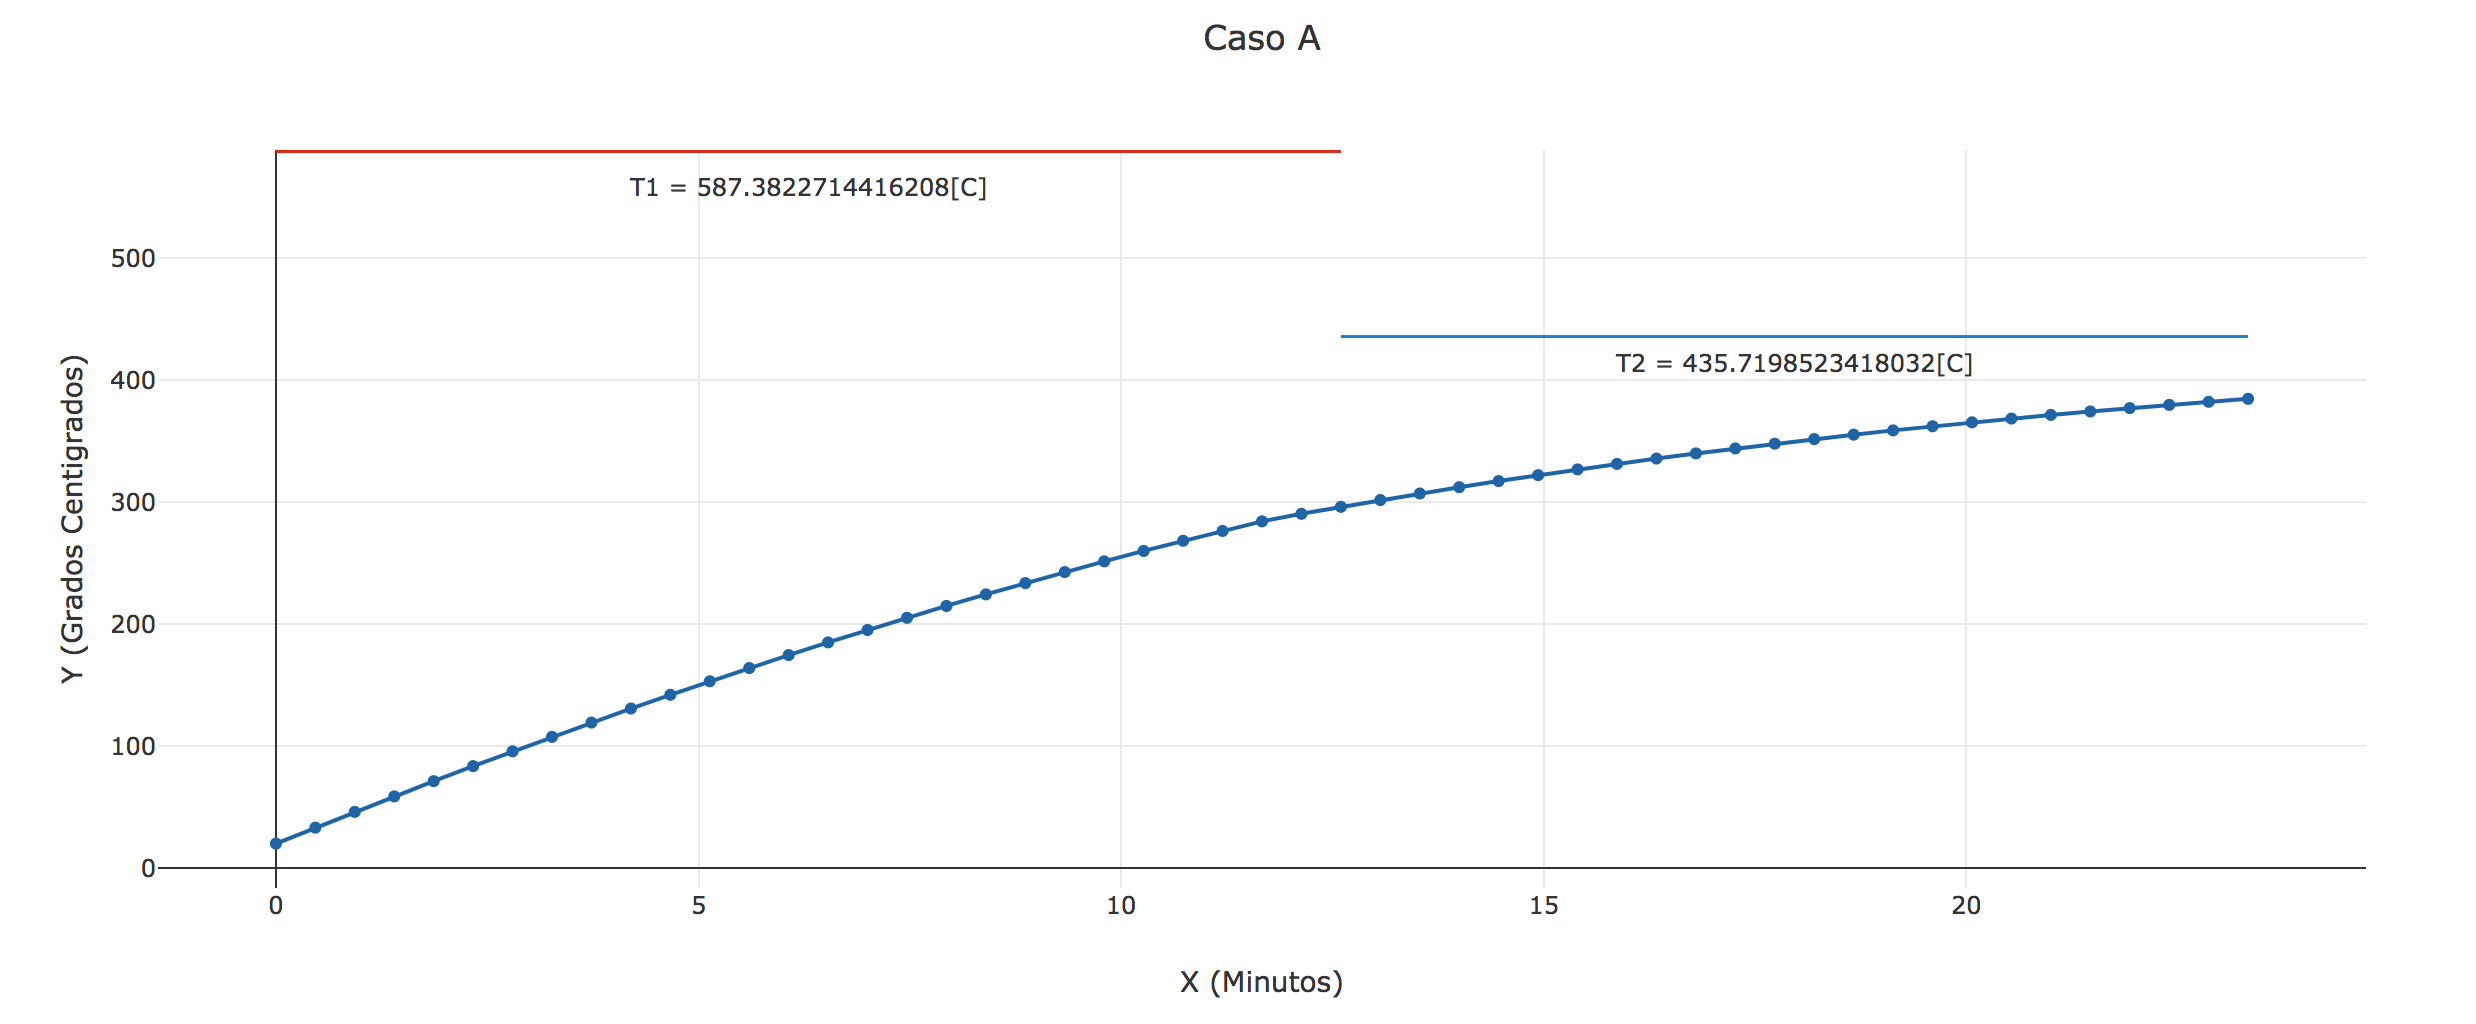
\includegraphics[width=18cm]{Grafica-ej5-casoa.png}
\caption{Gráfico para el caso A}
\end{figure}

\begin{figure}[H]
\centering
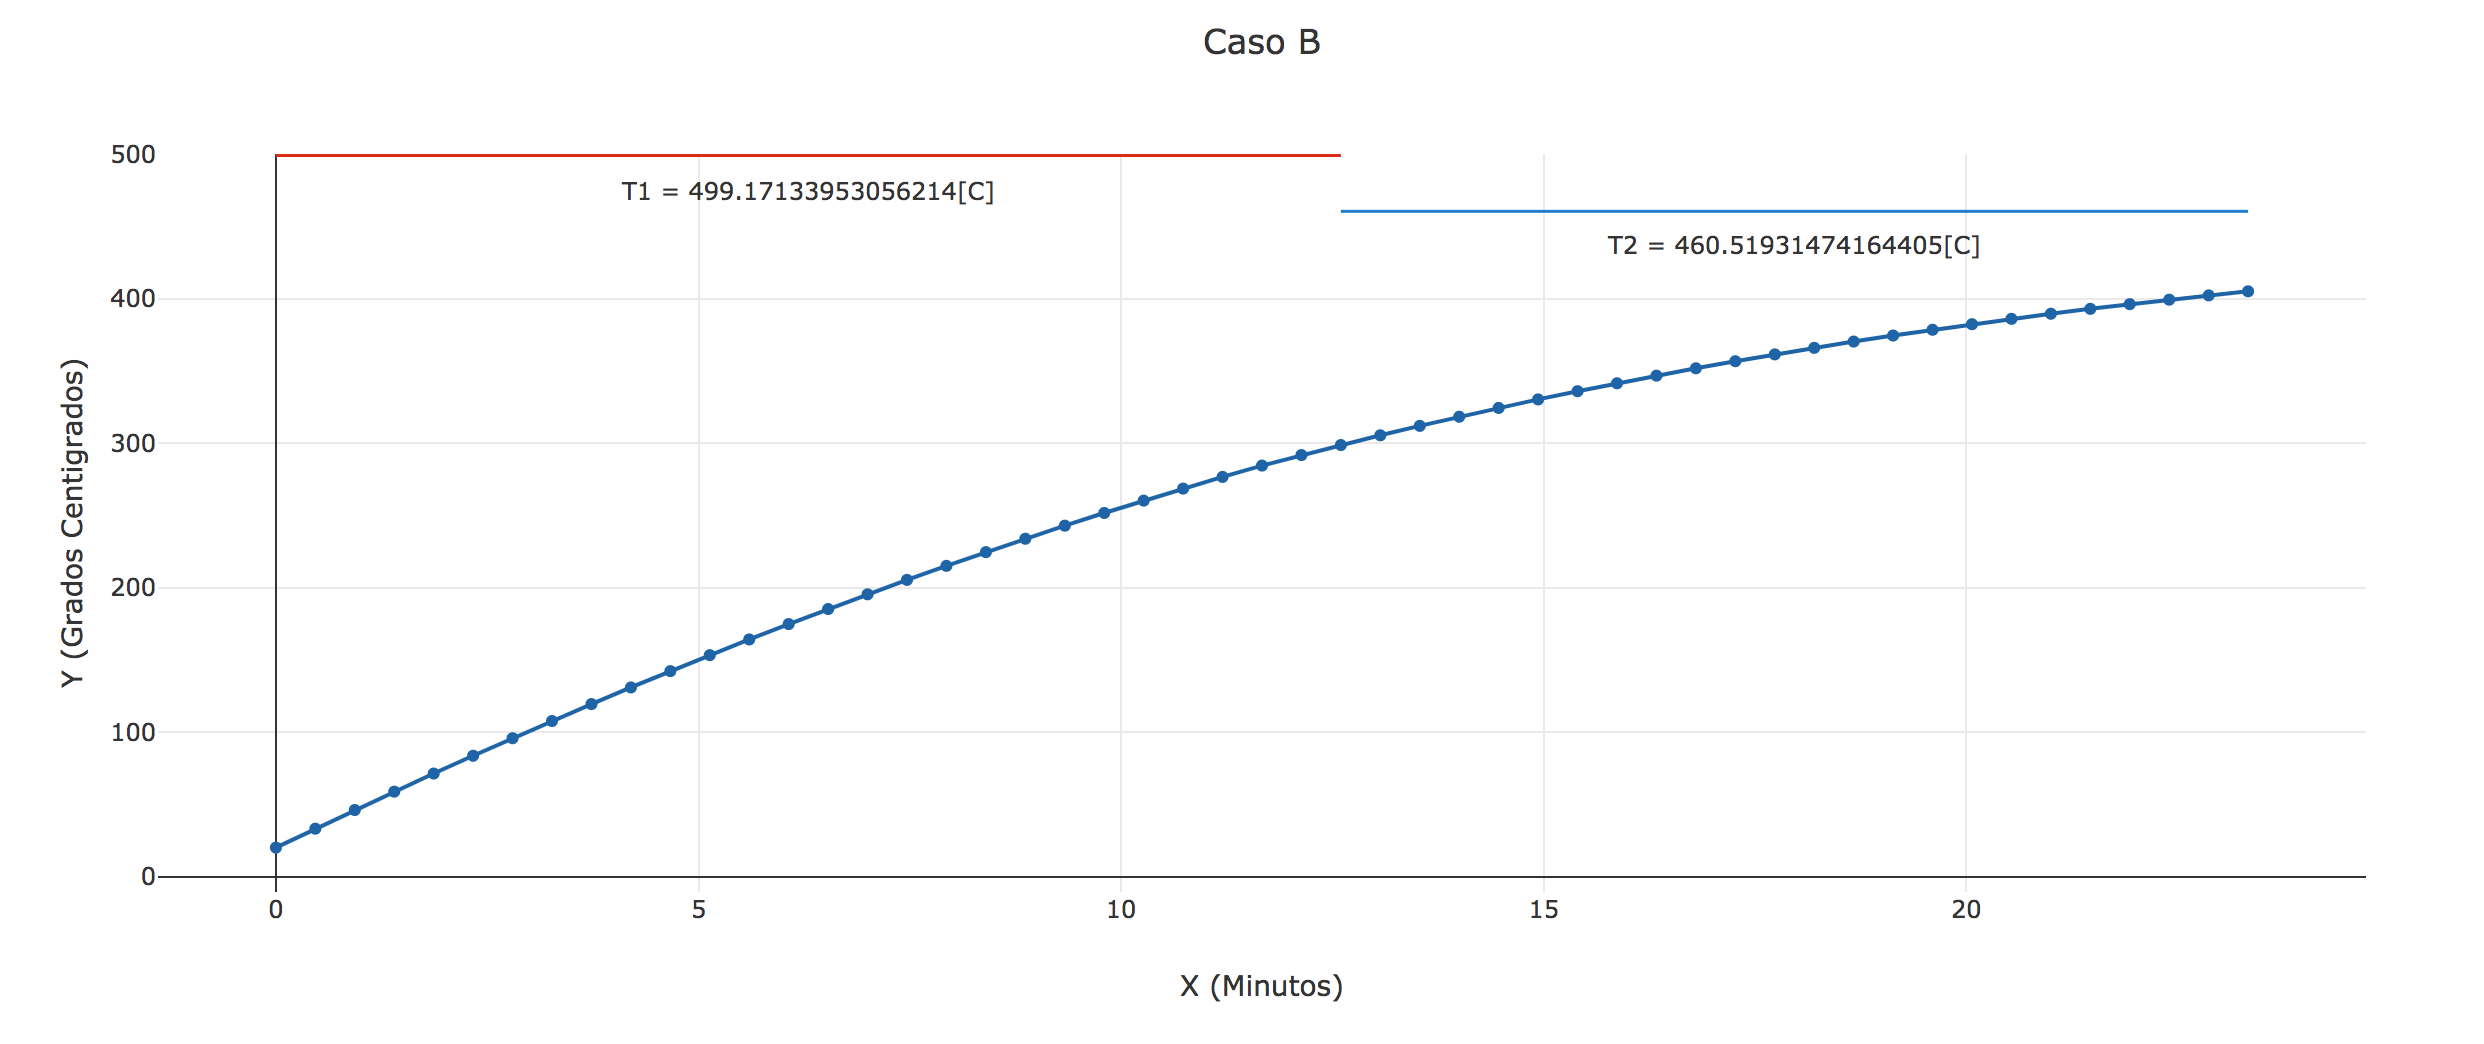
\includegraphics[width=18cm]{Grafica-ej5-casob.png}
\caption{Gráfico para el caso B}
\end{figure}

\begin{figure}[H]
\centering
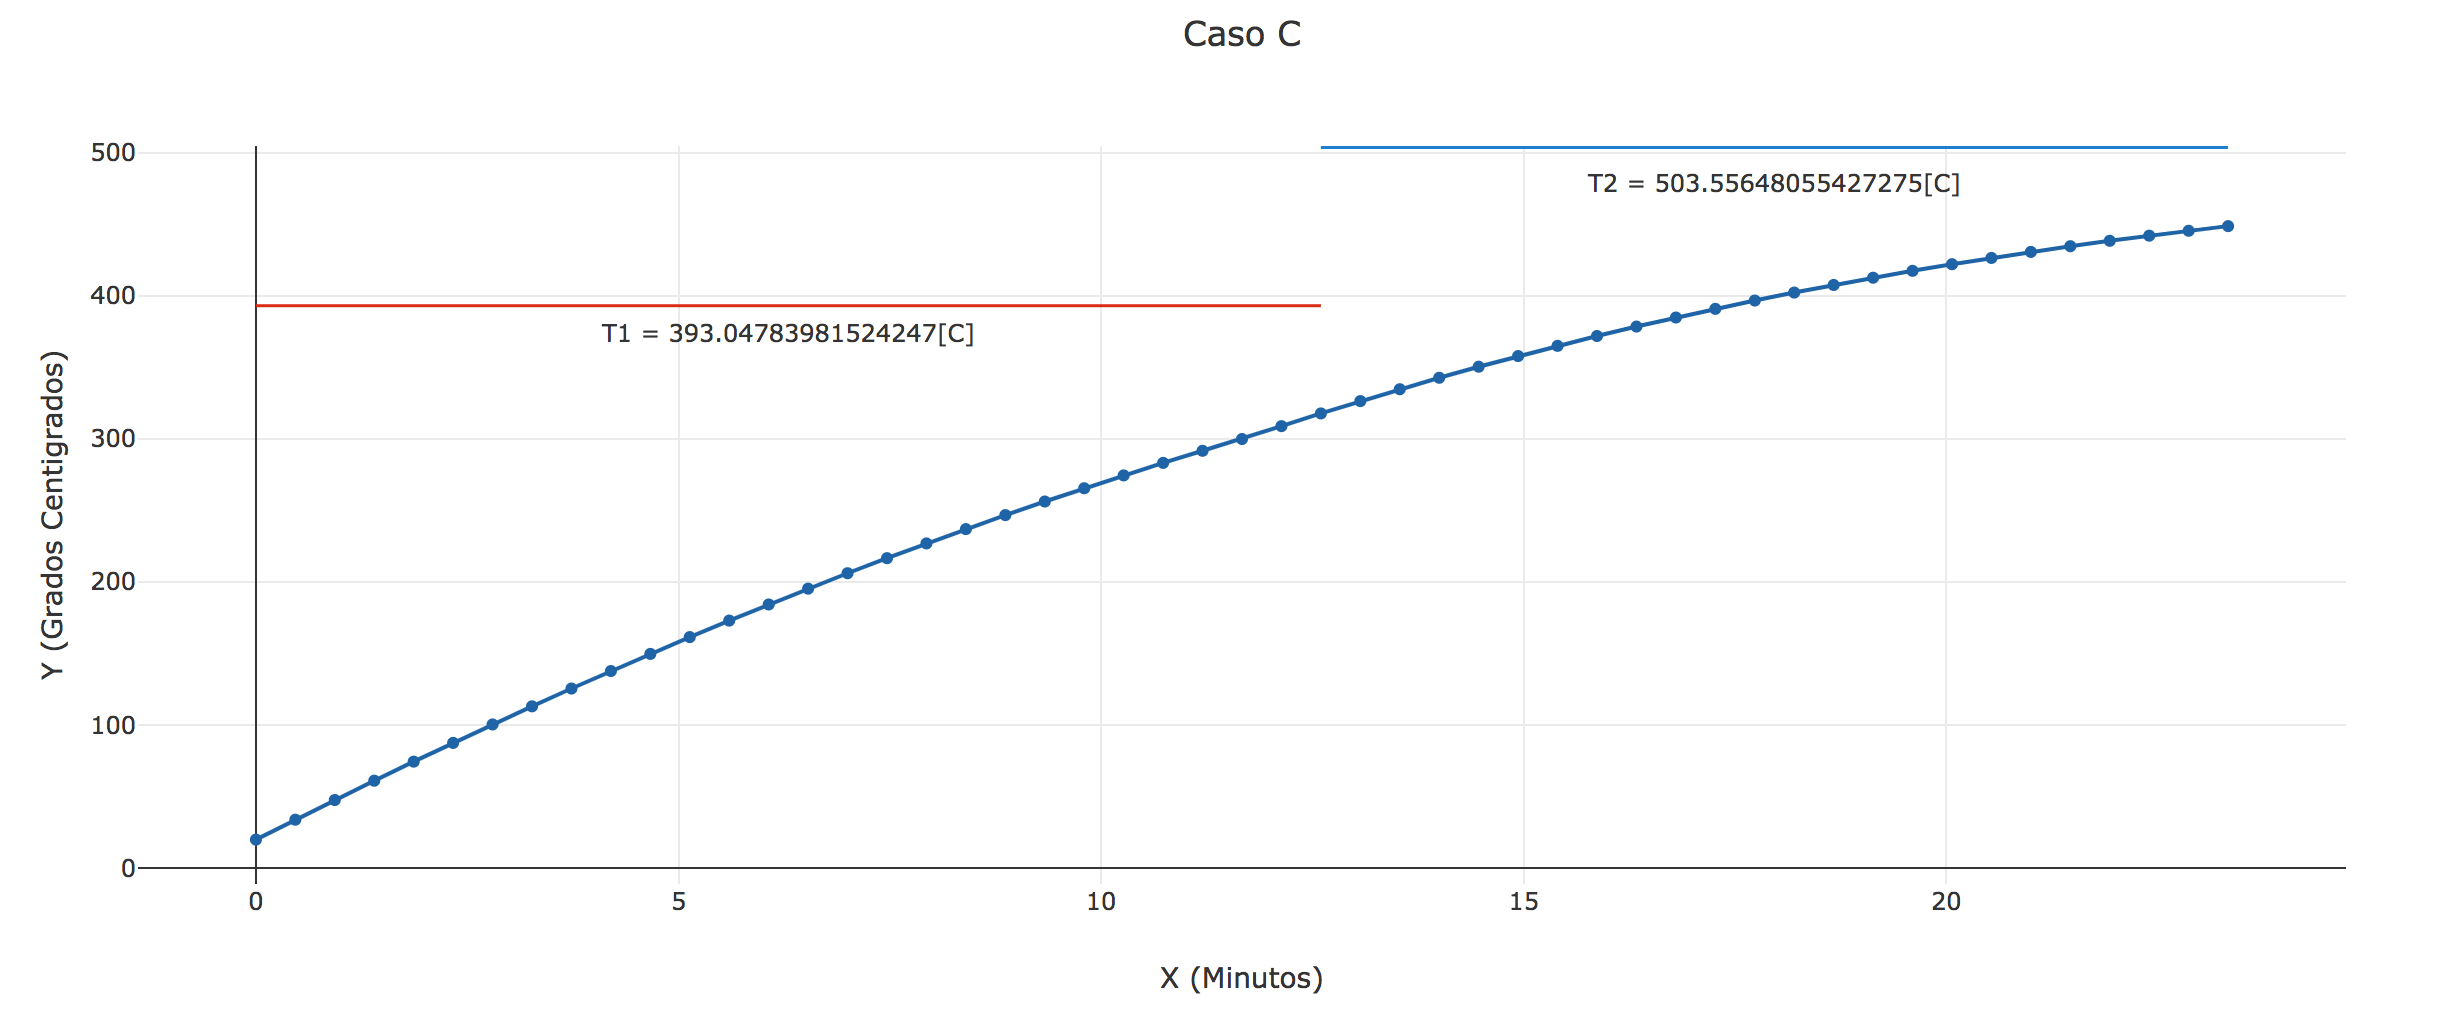
\includegraphics[width=18cm]{Grafica-ej5-casoc.png}
\caption{Gráfico para el caso C}
\end{figure}
\section{Conclusiones}

En este trabajo práctico han sido utilizados dos métodos de resolución de ecuaciones diferenciales para analizar el problema del revenido en la fabricación de tubos de acero con distintas necesidades mecánicas.\\

En un comienzo se uso únicamente el término referente al pasaje de calor mediante convección, el cual es una ecuación lineal. Para terminar de analizar el problema se le agregó a esta ecuación, el término correspondiente al pasaje de calor debido a la radiación, este término es exponencial.
De ambos modos, fueron resueltas las ecuaciones diferenciales pero la principal diferencia entre una y otra es la dificultad del despeje de la función solución.\\

En las ecuaciones diferenciales no lineales suele ser muy dificultoso o casi imposible el despeje a mano de la función a encontrar, debido a esto, los métodos numéricos sirven como una poderosa herramienta para hallar soluciones con una precisión aceptable a ecuaciones diferenciales no lineales.\\

En este caso, fueron utilizados los métodos numéricos para encontrar la solución a un problema inverso. Conociendo los valores de la imagen de la función, usarlos para así encontrar valores específicos de la preimagen de la misma. Esto es posible porque al ir aplicando cada uno de los métodos, quedan grabadas relaciones entre preimagen e imagen en una tabla, que pueden ser utilizadas a posteriori en el análisis.\\

Para acercarse mejor a la realidad, podría plantearse en la ecuación de conservación de energía, el calor debido al proceso de conducción. Ya que los tubos están apoyados sobre cada uno de los bolsillos, podría analizarse la pérdida o ganancia de calor referente al contacto entre el tubo y la superficie. \\


%----------------------------------------------------------------------------------------
%	BIBLIOGRAPHY
%----------------------------------------------------------------------------------------


\begin{thebibliography}{9}
\bibitem{youtube1} 
Algoritmo de Euler y Runge-Kutta de orden 2 para resolver una EDO
\\\texttt{https://www.youtube.com/watch?v=hgKzFdAZHwY}
\bibitem{wikirk}
Wikipedia - Método de Runge - Kutta
\\ \texttt{https://en.wikipedia.org/wiki/Runge\%E2\%80\%93Kutta\_methods}
\bibitem{wikieuler}
Wikipedia - Método de Euler
\\ \texttt{https://es.wikipedia.org/wiki/M\%C3\%A9todo\_de\_Euler}
\end{thebibliography}

%----------------------------------------------------------------------------------------


\end{document}
